\documentclass[12pt]{kiarticle}
\graphicspath{{pictures/}}
\DeclareGraphicsExtensions{.pdf,.png,.jpg,.eps}
%%%
\pagestyle{fancy}
\fancyhf{}
%\renewcommand{\headrulewidth}{ 0.1mm }
\renewcommand{\footrulewidth}{ .0em }
\fancyfoot[C]{\texttt{\textemdash~\thepage~\textemdash}}
\fancyhead[L]{Лабораторная работа №5.5 \hfil}
\fancyhead[R]{\hfil Иванов Кирилл, 625 группа }
\usepackage{multirow} % Слияние строк в таблице
\newcommand{\eds}{\ensuremath{ \mathscr{E}}}
\newcommand{\ga}{\ensuremath{\gamma}}
\usepackage{tikz}

%%% Работа с таблицами
\usepackage{array,tabularx,tabulary,booktabs} % Дополнительная работа с таблицами
\usepackage{longtable}  % Длинные таблицы
\usepackage{multirow} % Слияние строк в таблице

\begin{document}
	
	\begin{titlepage}
		\begin{center}
			\large 	Московский физико-технический институт \\
			(государственный университет) \\
			Факультет общей и прикладной физики \\
			\vspace{0.2cm}
			
			\vspace{4.5cm}
			Лабораторная работа №5.5  \\ \vspace{0.2cm}
			\large (Общая физика: квантовая физика) \\ \vspace{0.2cm}
			\LARGE \textbf{Компьютерная сцинтилляционная \ga-спектрометрия }
		\end{center}
		\vspace{2.3cm} \large
		
		\begin{center}
			Работу выполнил: \\
			Иванов Кирилл,
			625 группа
			\vspace{10mm}		
			
		\end{center}
		
		\begin{center} \vspace{60mm}
			г. Долгопрудный \\
			2018 год
		\end{center}
	\end{titlepage}


	\paragraph*{Цель работы:} да я блять не ебу 
	
	
	
	\section{Теоретическое введение}
	
	Основная задача спектрометрических измерений заключается в определении энергии, интенсивности дискретных гамма-линий от различных гамма-источников и их идентификации.
	
	Основными процессами взаимодействия гамма-излучения с веществом являются фотоэффект, эффект Комптона и образование электрон-позитронных пар. Каждый из этих процессов вносит свой вклад в образование наблюдаемого спектра. Образующиеся при этих процессах электроны испытывают большое количество неупругих соударений с молекулами и атомами среды. Неупругие соударения могут сопровождаться как ионизацией, так и возбуждением молекул или атомов среды. В промежуточных же стадиях (при переходах возбужденных молекул или атомов в основное состояние, при рекомбинации электрических зарядов и т.п.) в веществе возникают кванты света различных длин волн, присущих данному веществу.
	
	При \textbf{фотоэффекте} кинетическая энергия электрона $ T_e = E_\ga - I_i $, где $ I_i $ --- энергия ионизации $ i $-той оболочки атома. Фотоэффект особенно существенен для тяжелых веществ, где он идет с заметной вероятностью даже при высоких энергиях гамма-квантов. В легких веществах фотоэффект становится заметен лишь при относительно небольших энергиях гамма-квантов. Наряду с фотоэффектом, при котором вся энергия гамма-кванта передается атомному электрону, взаимодействие гамма-излучения со средой может приводить к его рассеянию, т.е. отклонению от первоначального направления распространения на некоторый угол.
	
	При \textbf{эффекте Компотна} происходит упругое рассеяние фотона на свободном электроне, сопровождающееся изменением длины волны фотона (реально этот процесс происходит на слабо связанных с атомом внешних электронах). Максимальная энергия образующихся комптоновских электронов соответствует рассеянию гамма-квантов на $ 2\pi $ и равна
	
	\begin{equation}\label{E_compton}
	E_{с \_ max} = \dfrac{\hbar \omega}{1 + \dfrac{m_ec^2}{2\hbar\omega}}
	\end{equation}
	
	При достаточно высокой энергии гамма-кванта наряду с фотоэффектом и эффектом Комптона может происходить третий вид взаимодействия гамма-квантов с веществом – \textbf{образование электрон-позитронных пар}. При этом если процесс образования пары идет в кулоновском поле ядра или протона, то энергия образующегося ядра отдачи оказывается весьма малой, так что пороговая энергия гамма-кванта, необходимая для образования пары, практически совпадает с удвоенной энергией покоя электрона $ Е_0 = 2m_ec^2 =1,022  $МэВ.
	
	Появившийся в результате процесса образования пар электрон теряет свою энергию на ионизацию среды. Таким образом, вся энергия электрона остается в детекторе. Позитрон будет двигаться до тех пор, пока практически не остановится, а затем аннигилирует с электроном среды, в результате чего появятся два гамма-кванта. Т.е., кинетическая энергия позитрона также останется в детекторе. Далее возможны три варианта развития событий:
	
	а) оба родившихся гамма-кванта не вылетают из детектора, и тогда вся энергия первичного гамма-кванта останется в детекторе, а в спектре появится пик с $ E = E_\gamma $;
	
	б) один из родившихся гамма-квантов покидает детектор, и в спектре появляется пик, соответствующий энергии $  Е = Е_\gamma - E0 $, где $ Е_0 = m_ec^2 = $ 511 кэВ;
	
	в) оба родившихся гамма-кванта покидают детектор, и в спектре появля- ется пик, соответствующий энергии $  Е = Е_\gamma - 2E0 $, где $ 2Е_0 = 2m_ec^2 = $ 1022 кэВ;
	
	Таким образом, любой спектр, получаемый с помощью гамма-спектрометра, описывается несколькими компонентами, каждая из которых связана с определенным физическим процессом. Как описано выше, основными физическими процессами взаимодействия гамма-квантов с веществом являются фотоэффект, эффект Комптона и образование электрон-позитронных пар, и каждый из них вносит свой вклад в образование спектра. Помимо этих процессов, добавляются экспонента, связанная с наличием фона, пик характеристического излучения, возникающий при взаимодействии гамма-квантов с окружающим веществом, а также пик обратного рассеяния, образующийся при энергии квантов $ Е_\gamma \gg mc^22/2 $ в результате рассеяния гамма-квантов на большие углы на материалах конструктивных элементов детектора и защиты. Положение пика обратного рассеяния определяется по формуле ($ E $ --- энергия фотопика):
	
	\begin{equation}\label{Eobr}
		E_{обр} = \dfrac{E}{1 + \dfrac{2E}{mc^2}}
	\end{equation}

%	\section{Экспериментальная установка}
%	
	Энергетическим разрешением спектрометра называется величина
	
	\begin{equation}\label{Ri = dE/E}
	R_i = \dfrac{\Delta E_i}{E_i}
	\end{equation}
	
	т.е. отношение ширины пика полного поглощения (измеренной на полувысоте) к регистрируемой энергии пика поглощения. Это значение $ E_i \propto \overline{n_i} $ --- числу частиц на выходе ФЭУ. При этом  $ \Delta E_i \propto \overline{\Delta n_i} = \sqrt{\overline{n_i}} $ --- ширина пика пропорциональна среднеквадратичной флуктуации, которая равна корню из числа частиц. Таким образом, наша формула \eqref{Ri = dE/E} примет вид
	
	\begin{equation}\label{Ri = c/E}
	R_i = \dfrac{\mathrm{const}}{E_i}
	\end{equation}
	
	\section{Выполнение работы}
	
	Проведем измерения гамма-спектров для $ \mathrm{^{22}Na, ^{137}Cs, ^{60}Co, ^{241}Am \;} и \mathrm{\; ^{152}Eu}$, а также измерение фона. Измерения для цезия повторим на соседней установке. Получаем зависимость счета на сцинтилляторе $ N'_ч $ от номера канала $ N $. 
	
	Найдем пики полного рассеяния для натрия $ \mathrm{^{22}Na} $ и цезия $ \mathrm{^{137}Cs} $:
	
	\begin{equation}\label{}
	N_{Na\_1} = 597,5, \quad N_{Na\_2} = 1395,2, \quad N_{Cs} =754,2
	\end{equation}
	
	Мы знаем, что этим пикам соответствуют табличные значения энергии 511, 1275 и 662 кэВ соответственно. Тогда проведем калибровку спектрометра, построив линейную зависимость энергии гамма-кванта от номера канала $ E_j = f(N_j) $. Результат калибровки:
	
	\begin{equation}\label{}
	E_j = (-60.537 + 0.957N_i ) \; кэВ
	\end{equation}
	
	С помощью полученной зависимости переведем все полученные значения каналов в энергии, а счет сцинтиллятора отнормируем по времени, получив число частиц за секунду $ N_ч = \dfrac{N'_ч}{t} $. Погрешность счета подсчитаем по формуле 
	
	 \begin{equation}\label{}
	\sigma_{N_ч} = N_ч \x \dfrac{\sqrt{N'_ч}}{N'_ч} = \dfrac{\sqrt{N'_ч}}{t}
	\end{equation}
	
	Во всех измерениях $ t $ в диапазоне 600 -- 700 секунд. Отложим по оси абсцисс энергию полученных экспериментальных точек, а по оси ординат -- число частиц за секунду (рис. 1 -- 6).
	
	С помощью ПО компьютера экспериментальной установки получим значения пиков полного поглощения и их ширины. По формуле \eqref{Ri = dE/E} подсчитаем для них разрешающую способность спектрометра. Результаты сведем в таблицу.
	
	\begin{figure}[H]
		\label{graf_bg}
		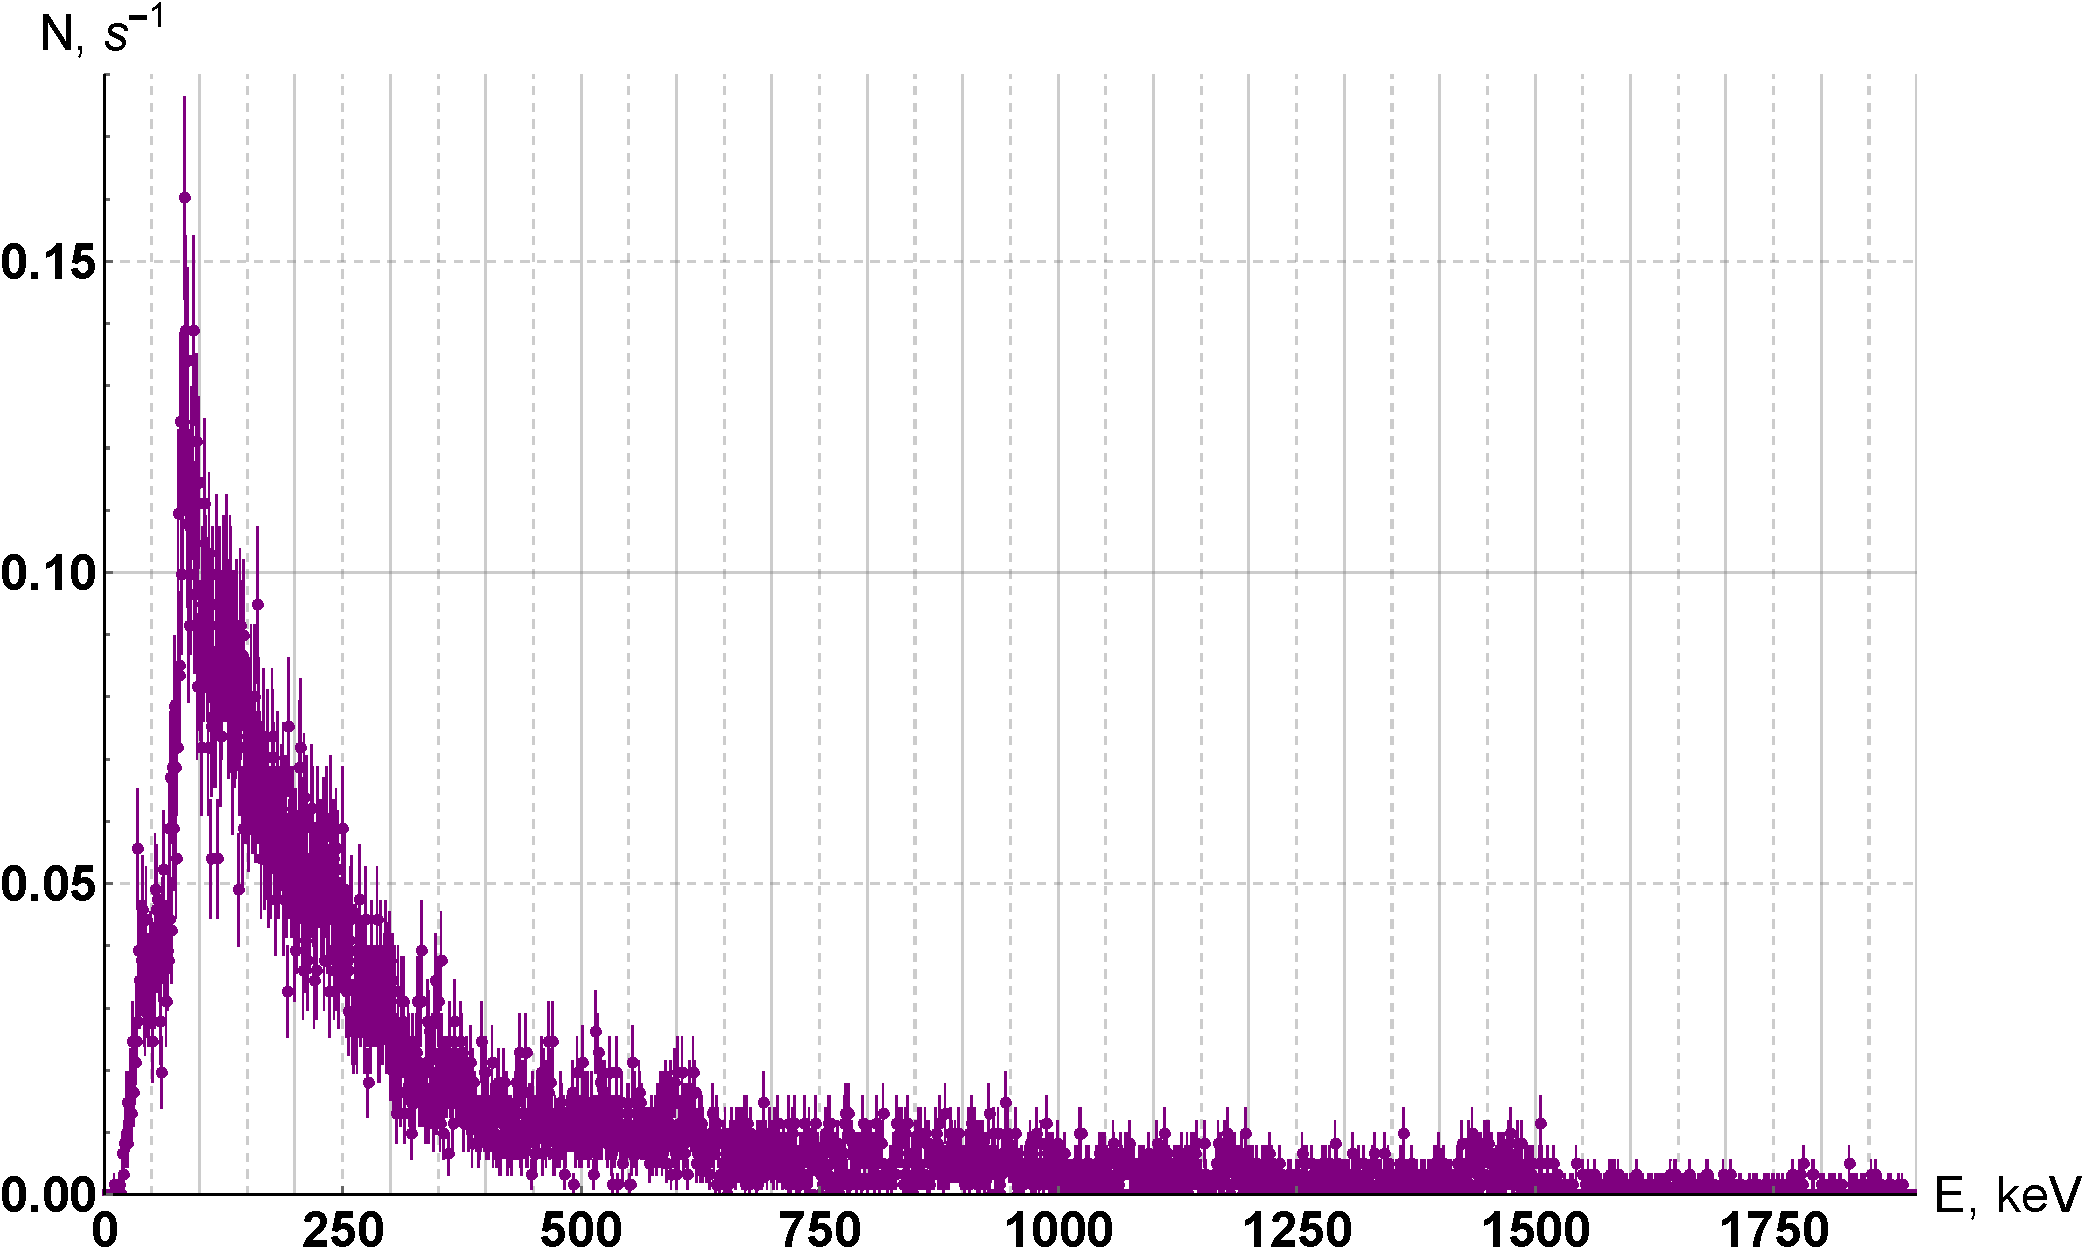
\includegraphics[scale=0.5]{bg.pdf}
		\caption{Измерение фона}
	\end{figure} 	
	
	\begin{figure}[H]
		\label{graf_na}
		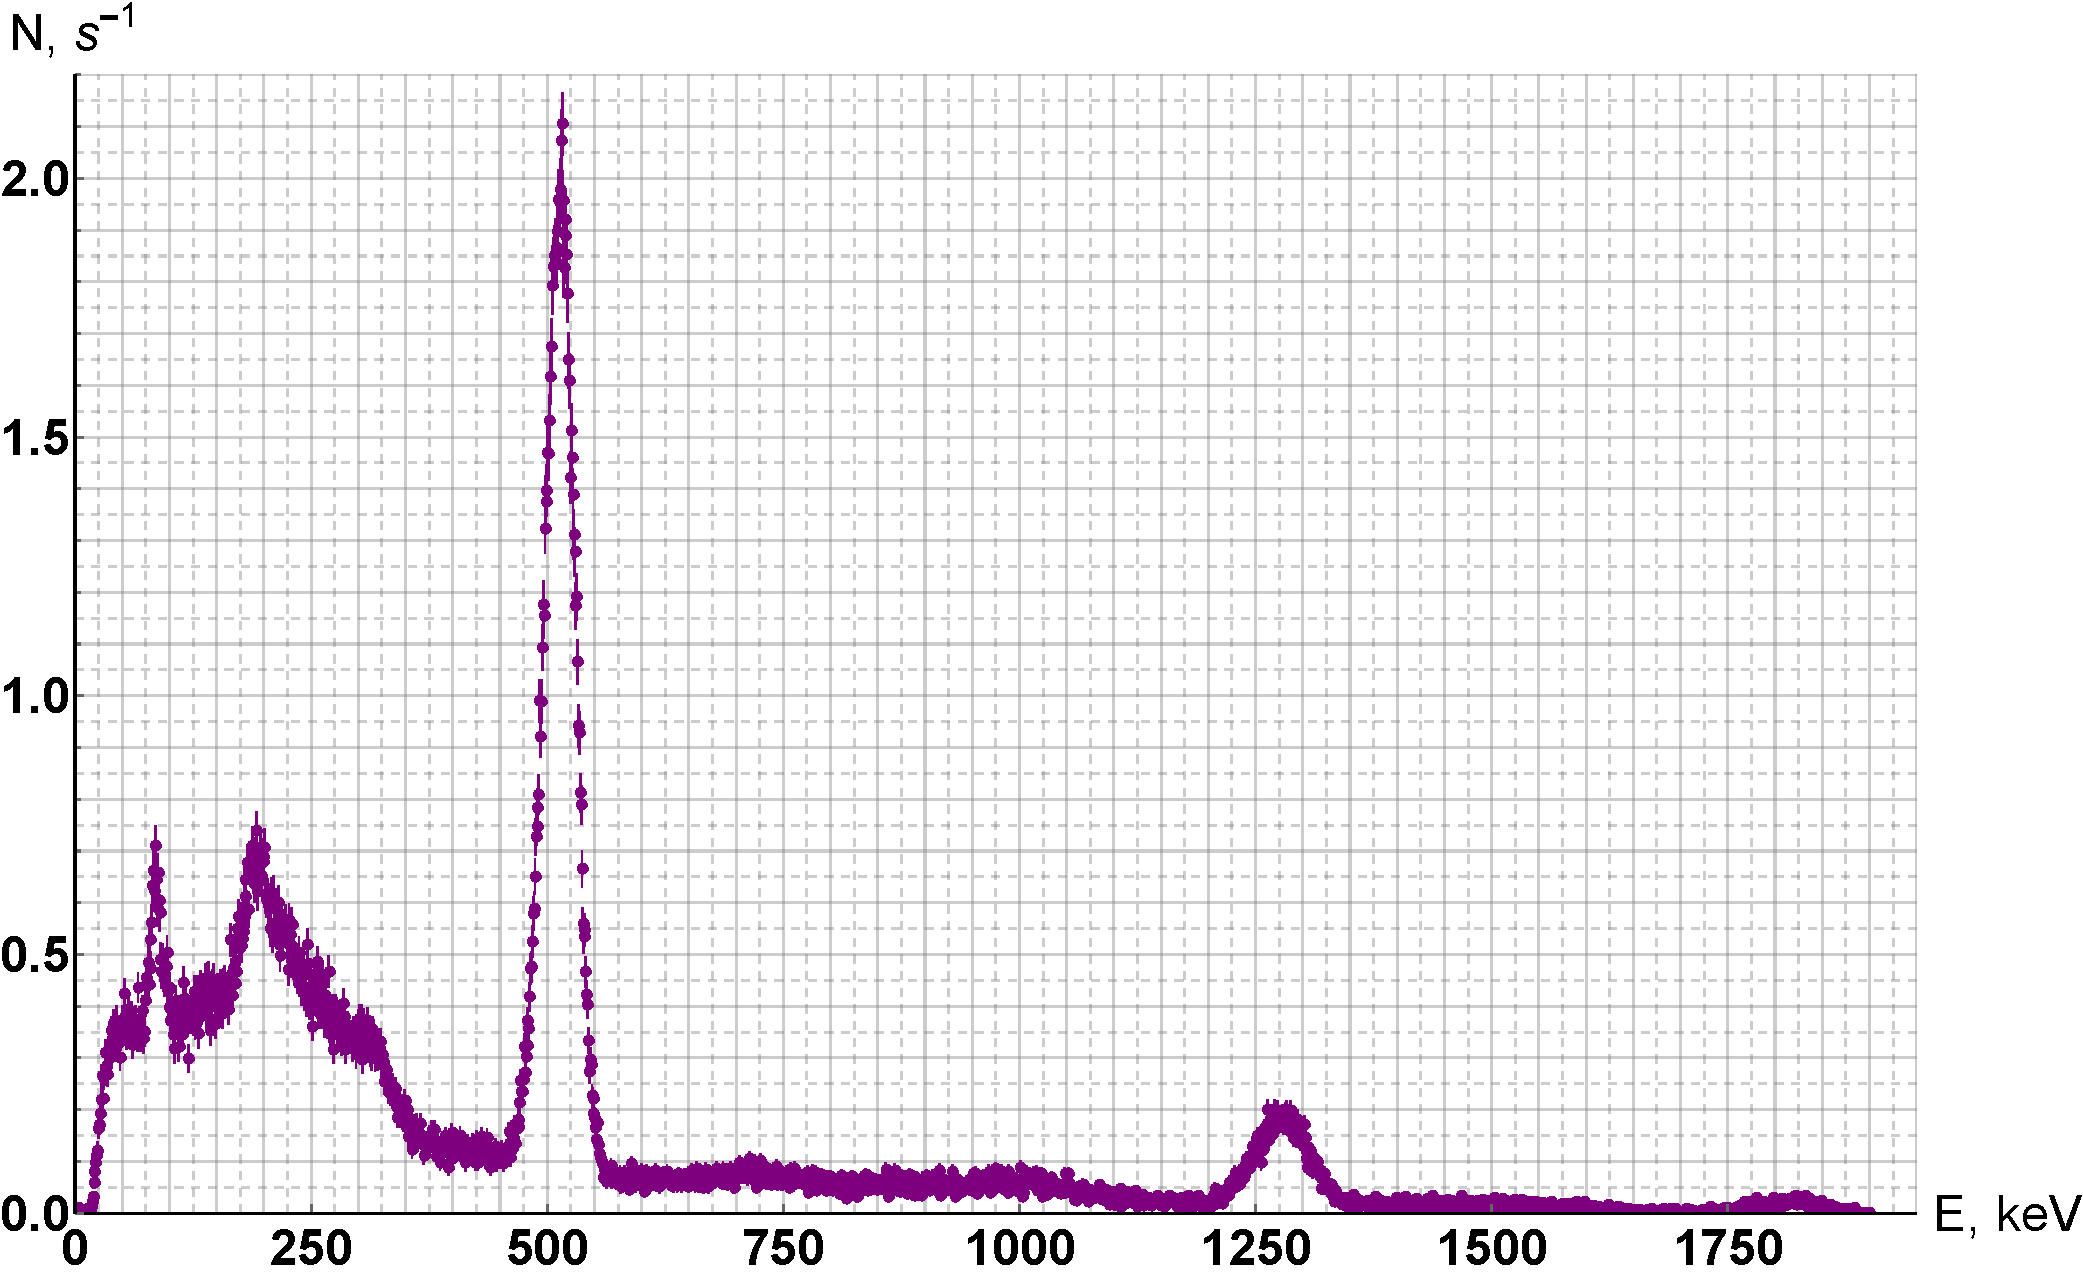
\includegraphics[scale=0.5]{na.pdf}
		\caption{Измерение спектра источника натрия $ \mathrm{^{22}Na} $}
	\end{figure} 

\begin{figure}[H]
	\label{graf_co}
	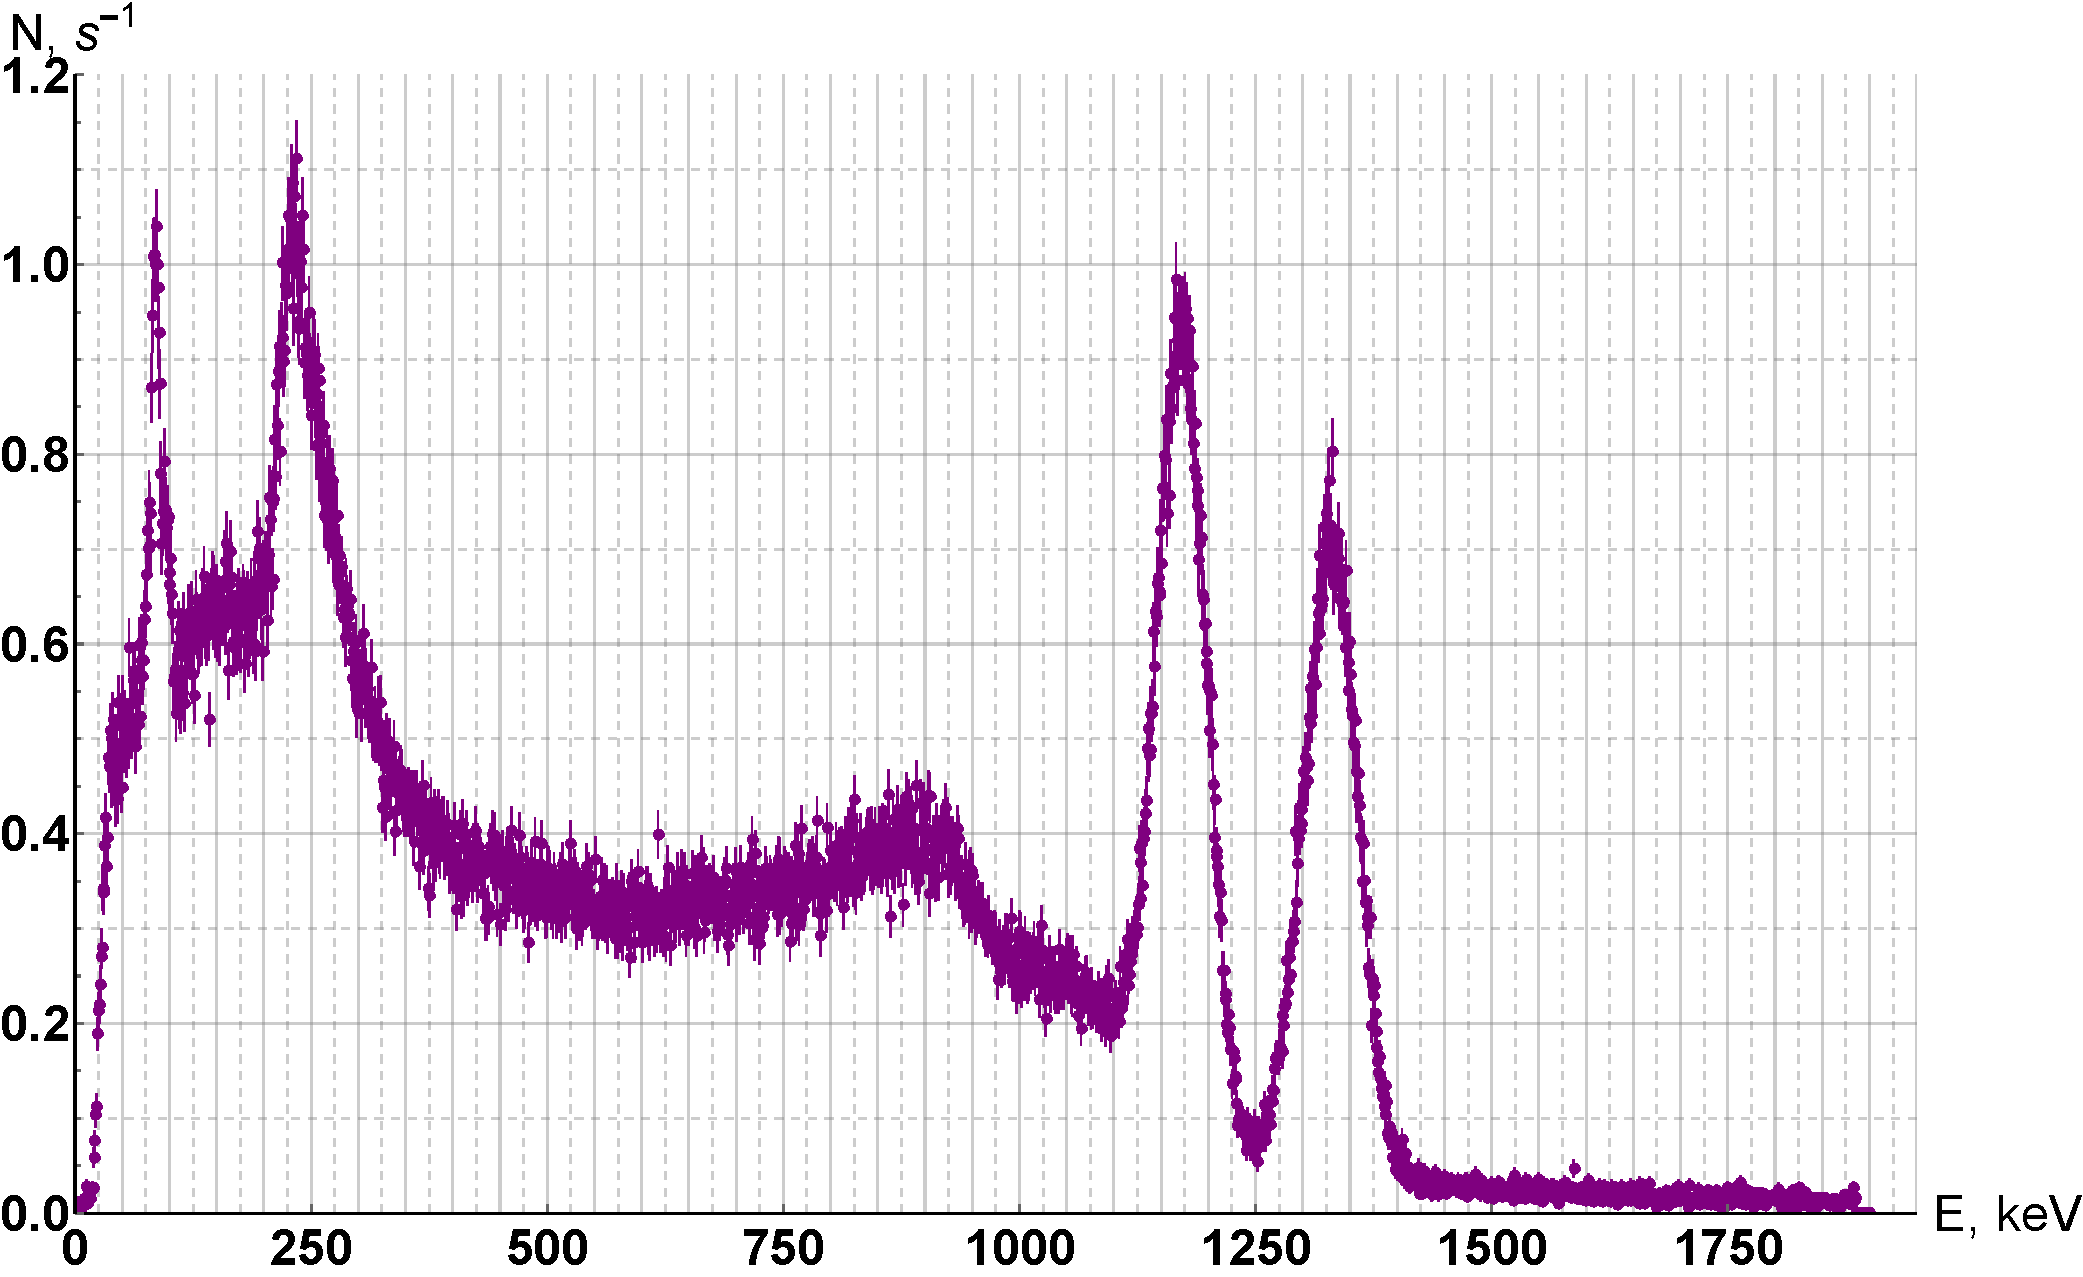
\includegraphics[scale=0.5]{co.pdf}
	\caption{Измерение спектра источника кобальта $ \mathrm{^{60}Co} $}
\end{figure} 

	\begin{figure}[H]
	\label{graf_cs}
	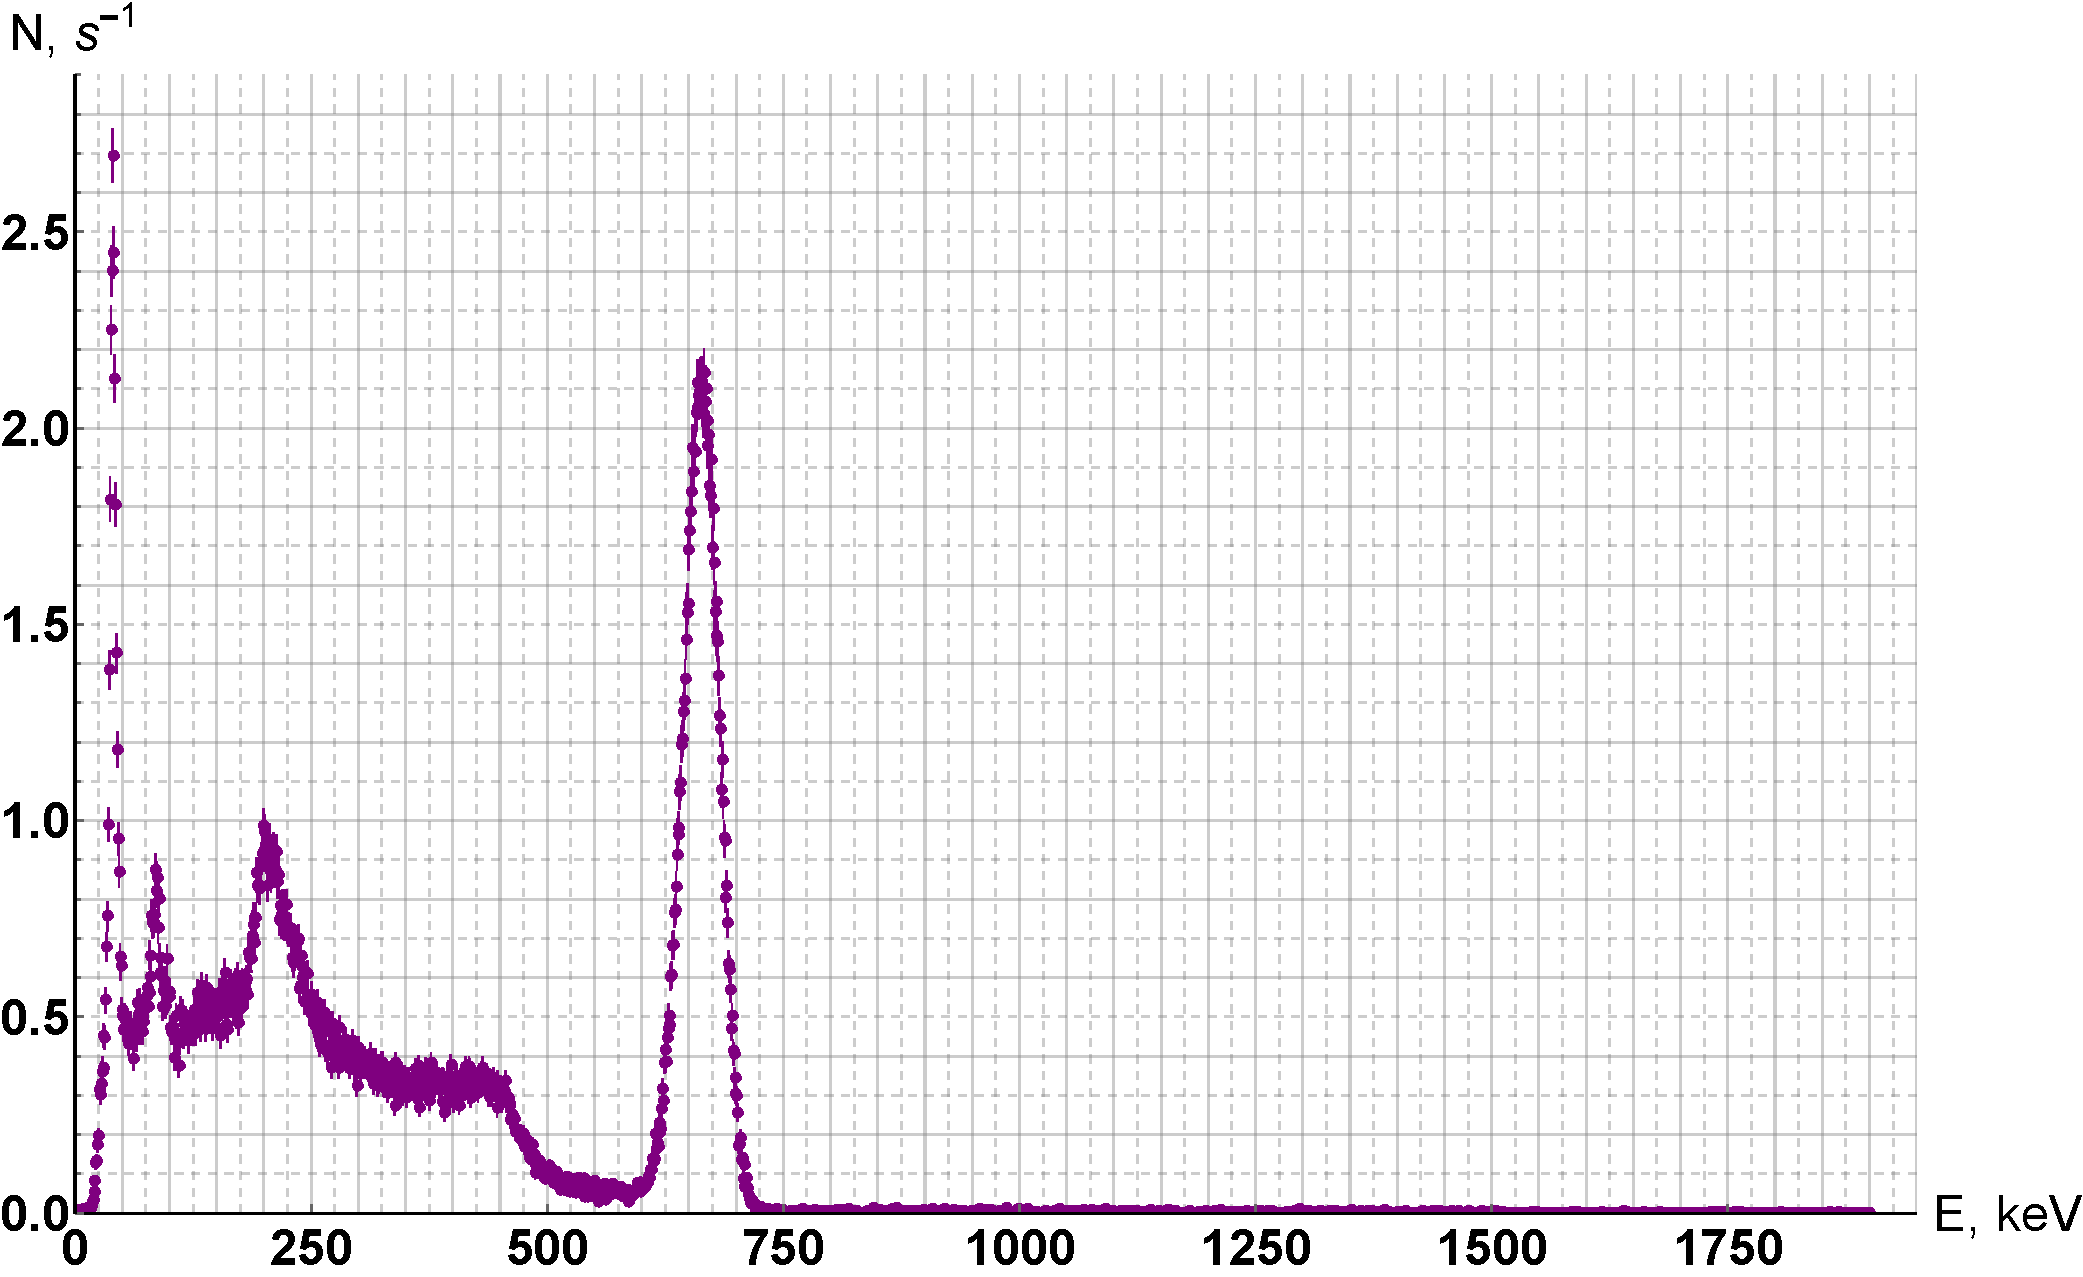
\includegraphics[scale=0.5]{cs.pdf}
	\caption{Измерение спектра источника цезия $ \mathrm{^{137}Cs} $}
\end{figure} 

\begin{figure}[H]
	\label{graf_cs2}
	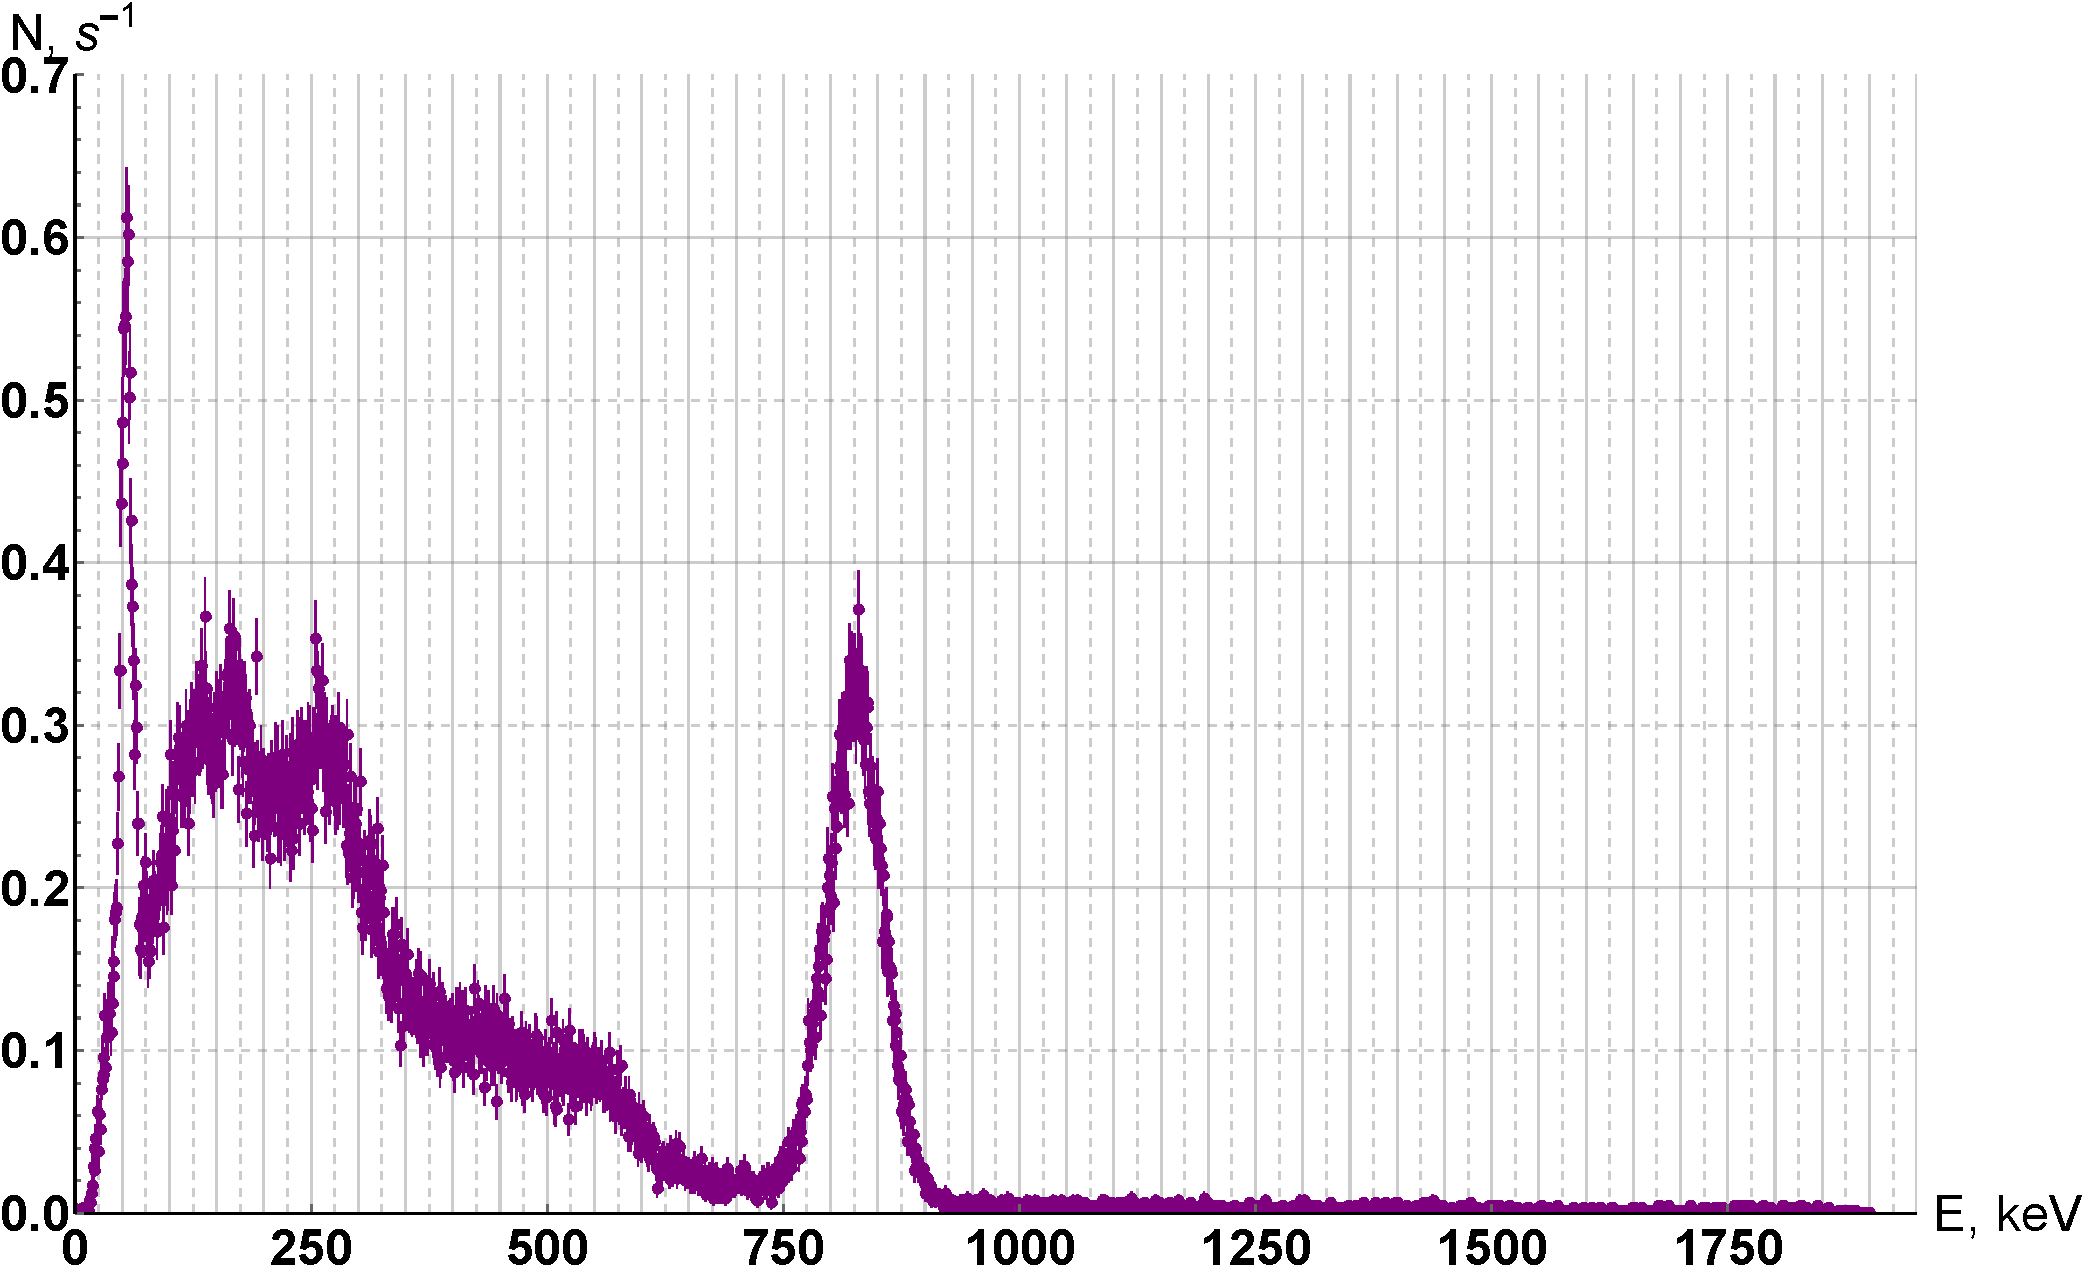
\includegraphics[scale=0.5]{cs2.pdf}
	\caption{Измерение на второй установке спектра источника цезия $ \mathrm{^{137}Cs} $} 
\end{figure} 

\begin{figure}[H]
	\label{graf_am}
	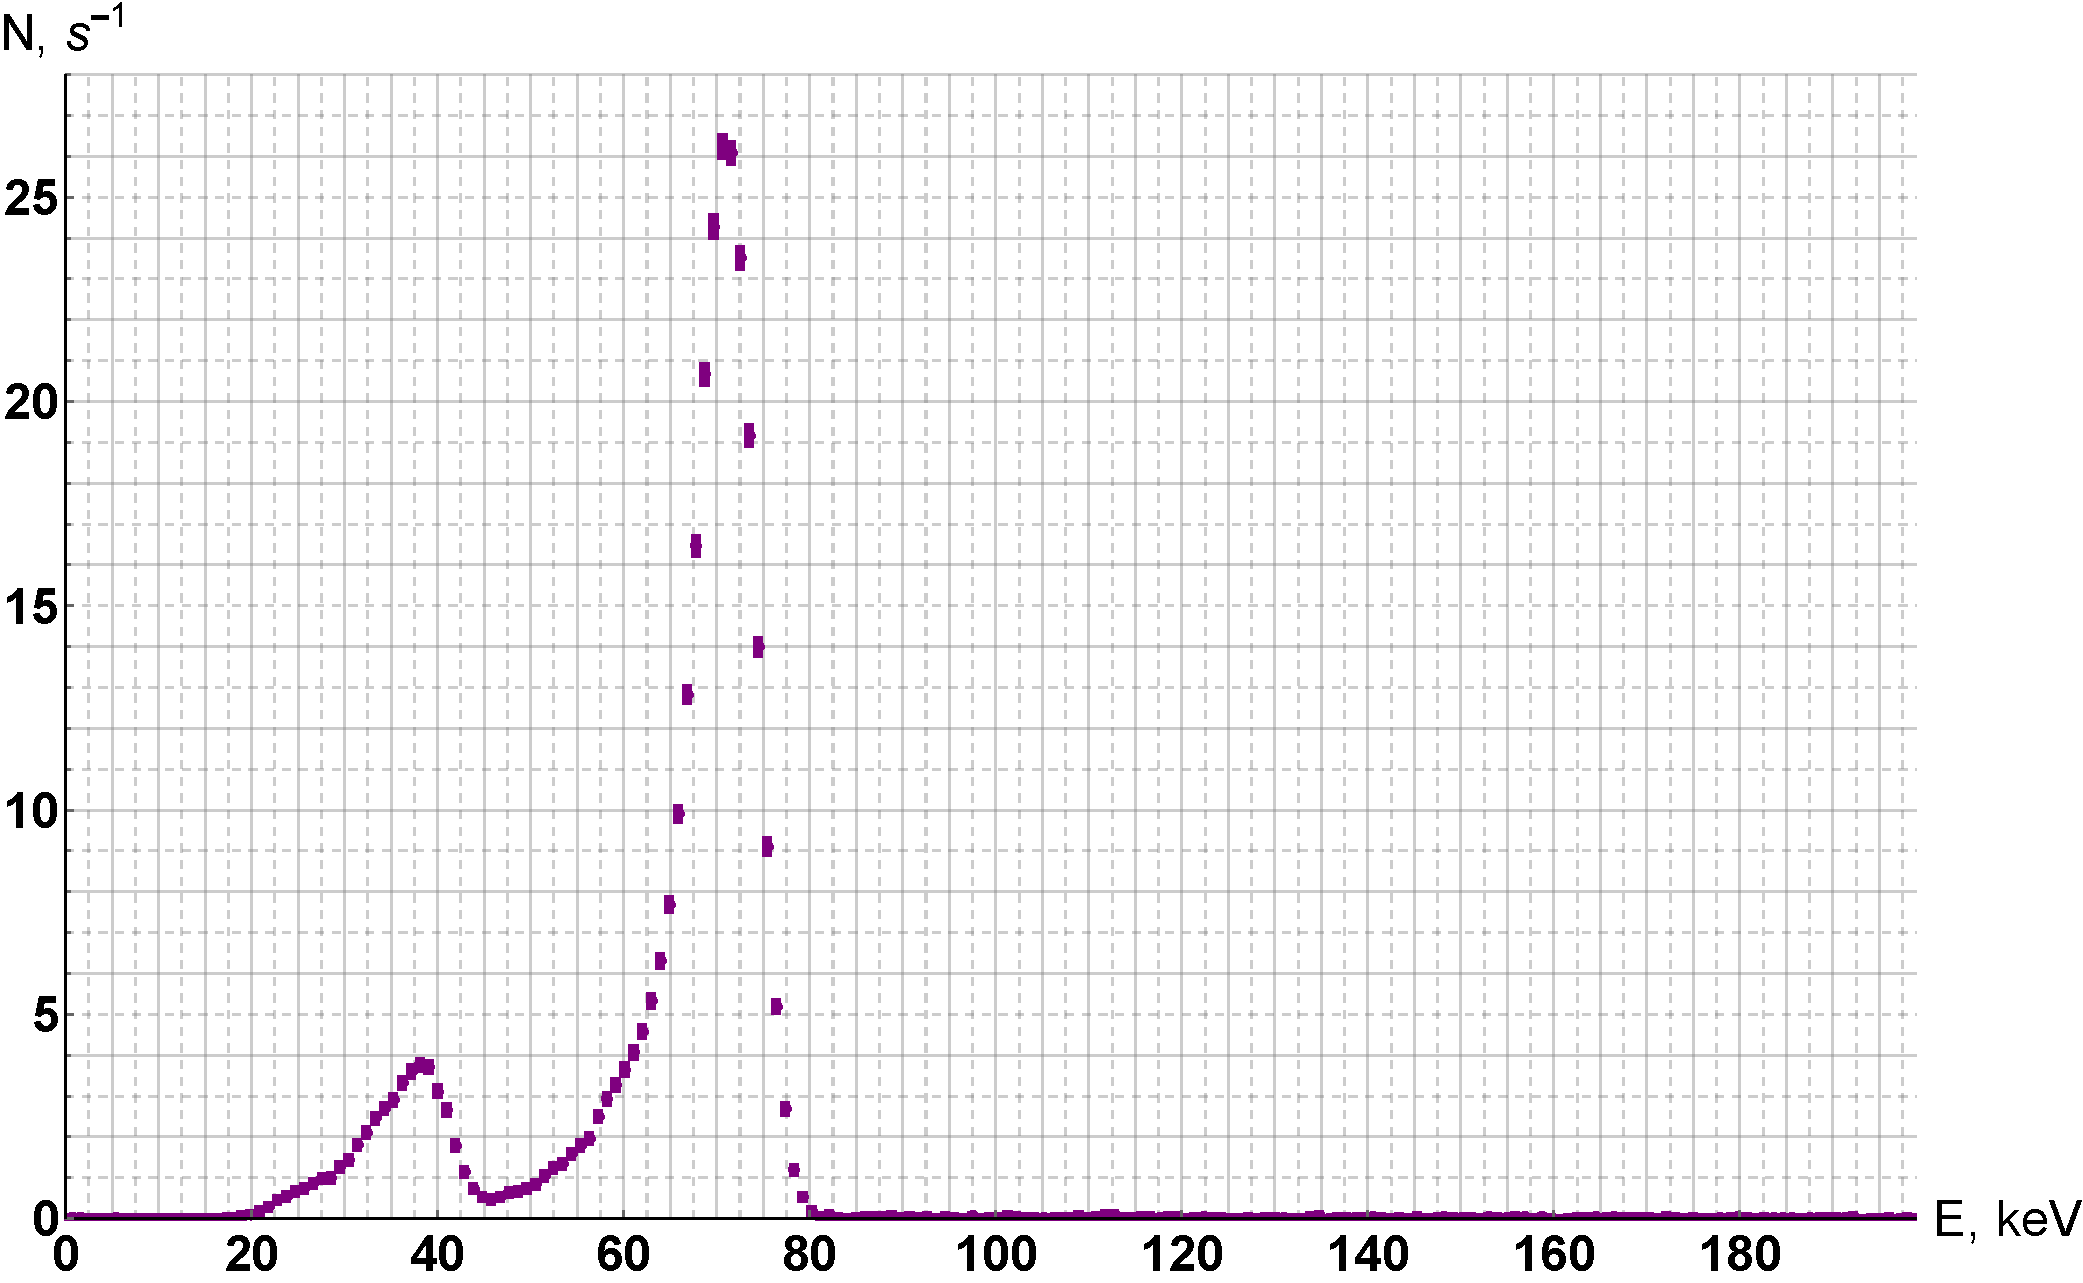
\includegraphics[scale=0.5]{am.pdf}
	\caption{Измерение спектра источника америция $ \mathrm{^{241}Am} $}
\end{figure} 

\begin{figure}[H]
	\label{graf_eu}
	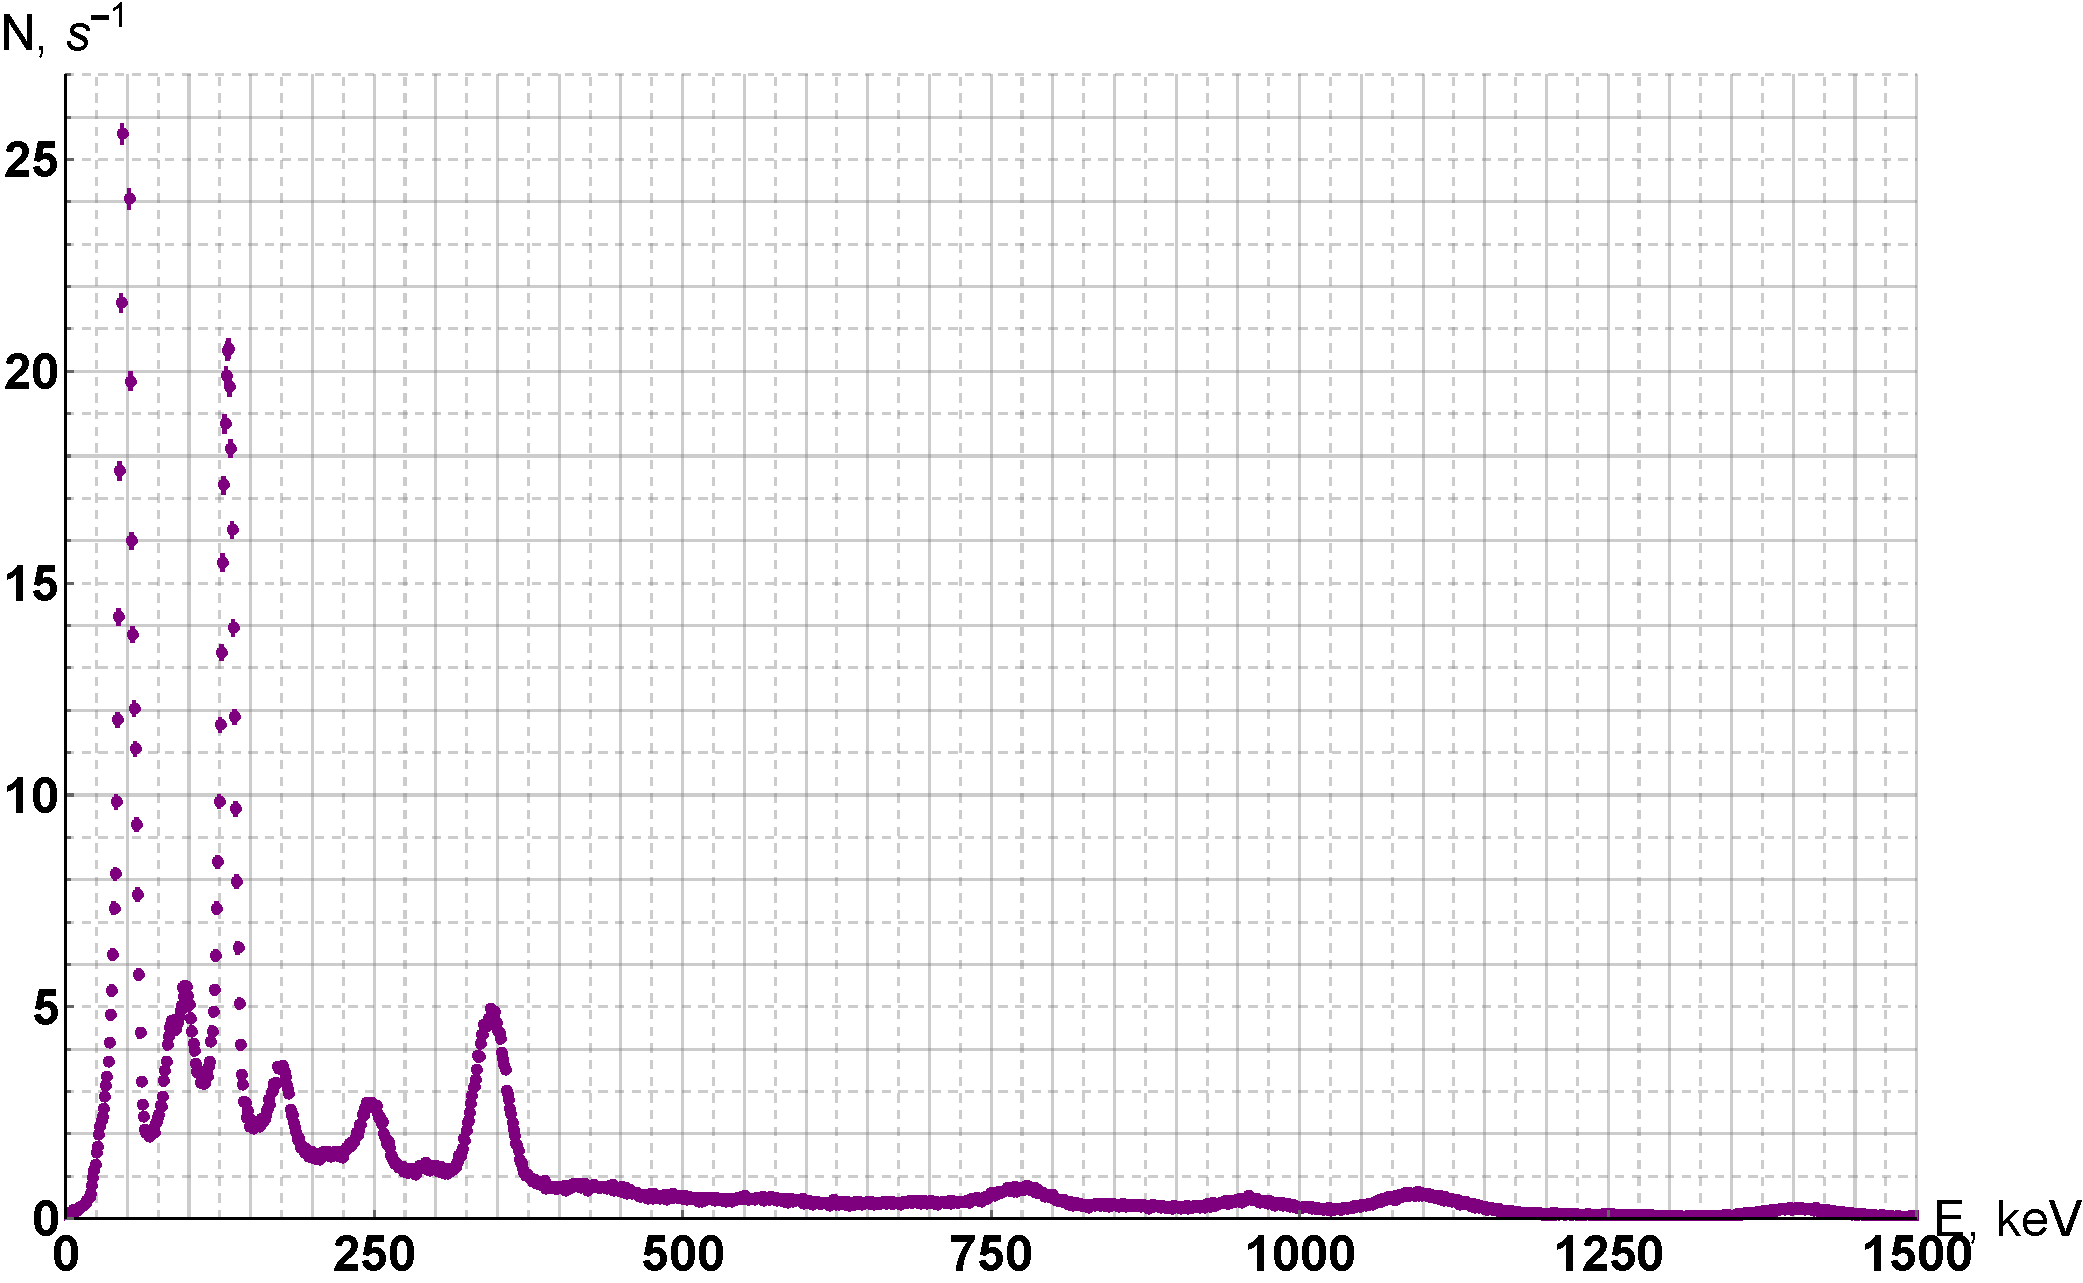
\includegraphics[scale=0.5]{eu.pdf}
	\caption{Измерение спектра источника европия $ \mathrm{^{152}Eu} $}
\end{figure} 
	
	
	\begin{table}[H]
		\caption{Пики прямого поглощения}
		\begin{center}
			\begin{tabular}{|c|c|c|c|c|c|}
				\hline 
				Образец & $N_i $ & $ \Delta N_i $ & $ E_i, $ кэВ & $ \Delta E,_i $ кэВ  & $ R_i $ \\ 
				\hline 
				Натрий $ \mathrm{^{22}Na} $ & 597.48 & 42 & 511.4 & 40.2 & 0.079 \\
				Натрий $ \mathrm{^{22}Na} $& 1395.23 & 76.6 & 1275.1 & 73.4 & 0.058 \\
				Цезий $ \mathrm{^{137}Cs} $ & 754.22 & 47.4 & 661.5 & 45.3 & 0.069 \\
				Кобальт $ \mathrm{^{60}Co} $ & 1286.1 & 65.1 & 1170.6 & 62.3 & 0.053 \\
				Кобальт $ \mathrm{^{60}Co} $ & 1450.59 & 73.3 & 1328.1 & 70.2 & 0.053 \\
				Америций $ \mathrm{^{241}Am} $& 135.57 & 9.5 & 69.2 & 9 & 0.131 \\
				Европий	 $ \mathrm{^{152}Eu} $& 199.01 & 12.3 & 130 & 11.7 & 0.09 \\
				Европий	 $ \mathrm{^{152}Eu} $& 421.7 & 30.4 & 343.2 & 29.1 & 0.085 \\
				\hline 
			\end{tabular} 
		\end{center}
		\label{res}
	\end{table}

	Экспериментально оценим пики комптоновского рассеяния и сравним с теоретическим расчетом. Результаты сведем в таблицу. Построим график зависимости теоретического расчета от экспериментального. 
	
	\begin{figure}[H]
		\label{graf_com}
		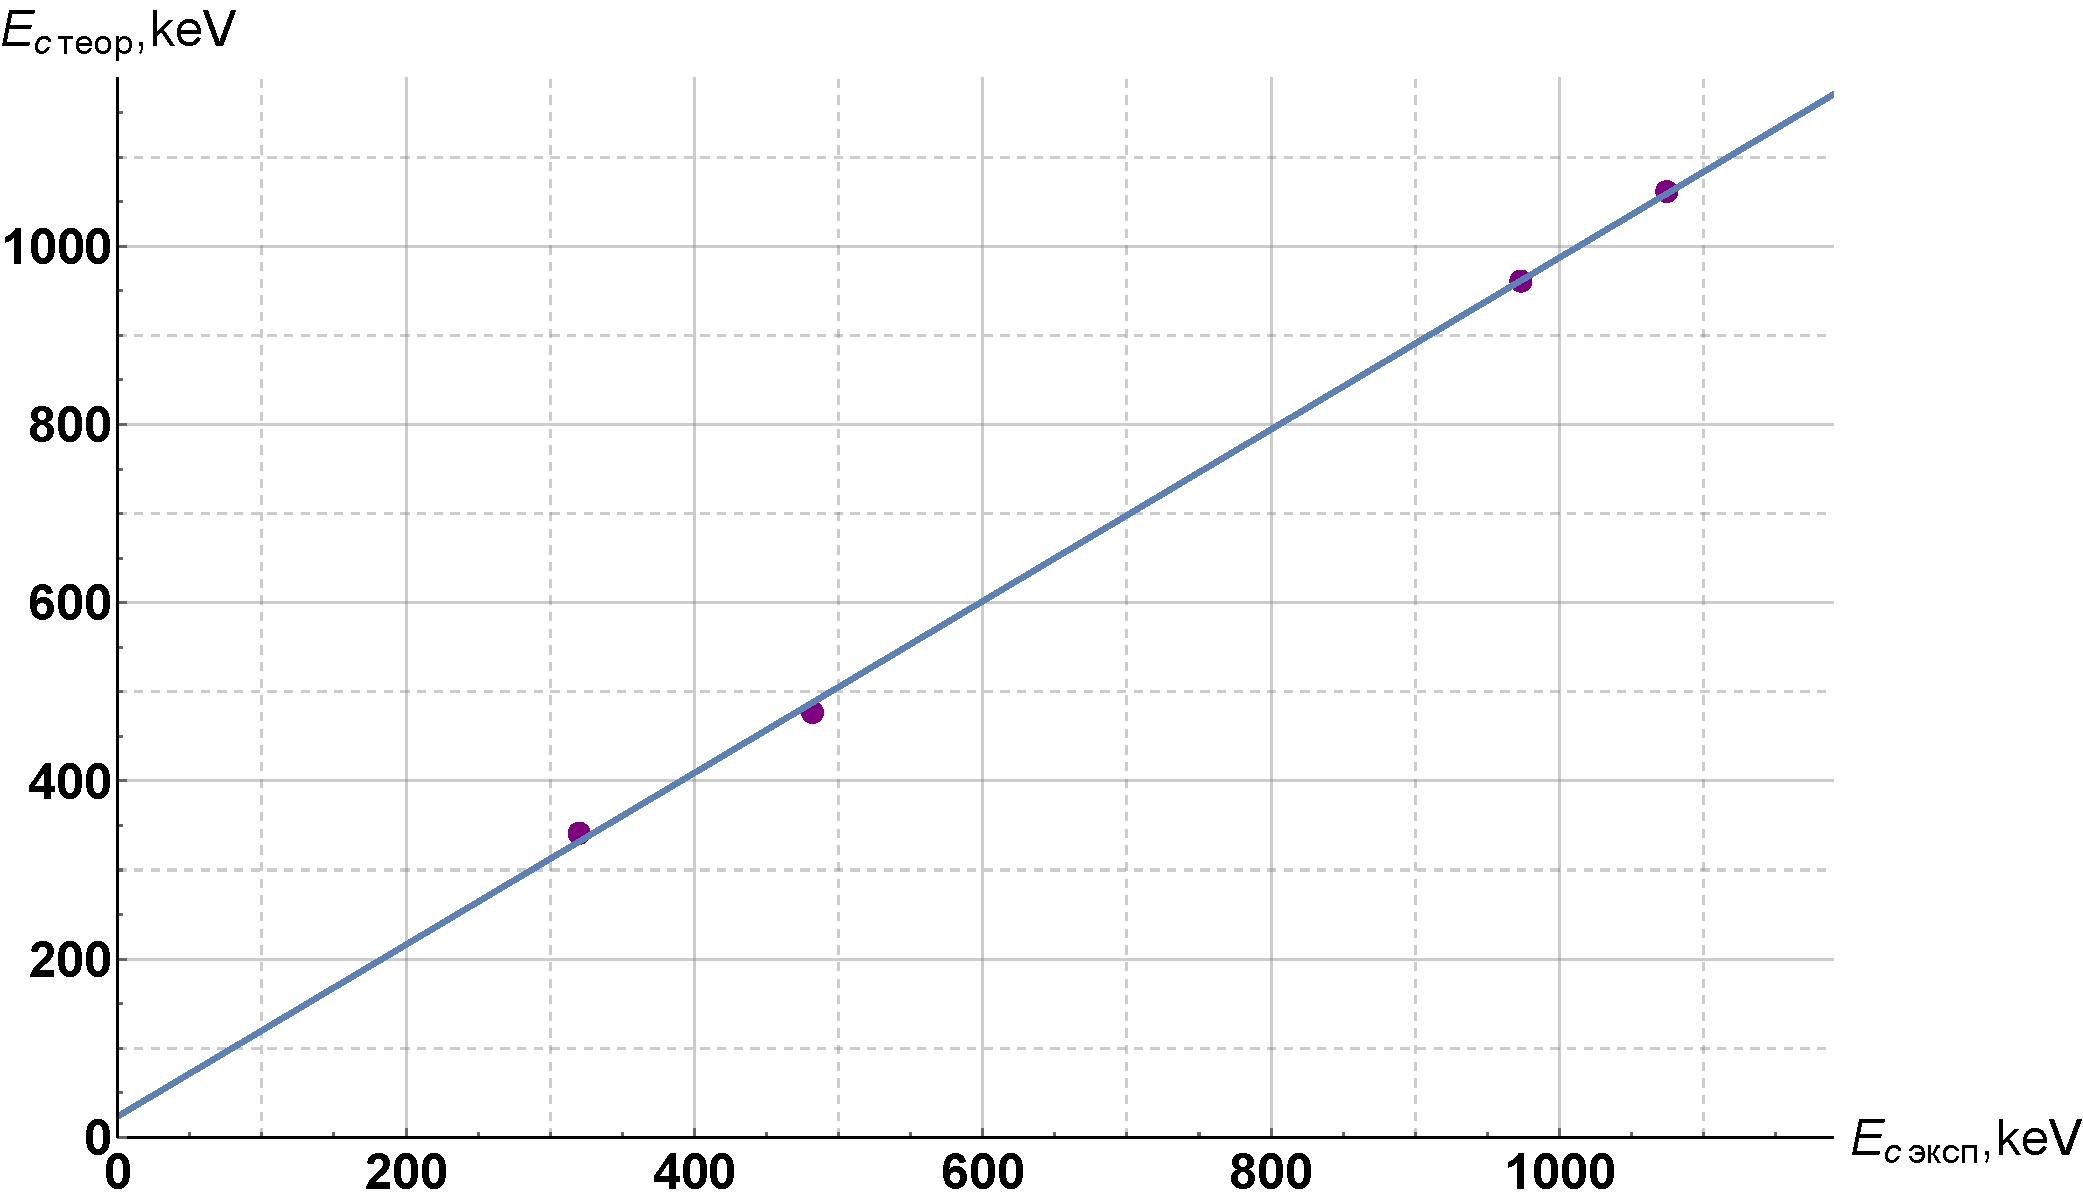
\includegraphics[scale=0.5]{comp.pdf}
		\caption{Зависимости теоретического расчета края комптоновского спектра от экспериментального}
	\end{figure} 
	
		Найдем параметры фита: 
	
	\begin{table}[H]
		\caption{Комптновские спектры}
		\begin{center}
			\begin{tabular}{|c|c|c|c|}
				\hline 
				Образец & $ E_i, $ кэВ  & $ E_{c\; экс}, $ кэВ  & $ E_{c \; теор}, $ кэВ \\
				\hline 
		Натрий $ \mathrm{^{22}Na} $ & 511.4 & 320.5 & 341. \\
		Цезий $ \mathrm{^{137}Cs} $ & 661.5 & 482.2 & 477.2 \\
		Кобальт $ \mathrm{^{60}Co} $ & 1270.6 & 973.3 & 960.9 \\
			Натрий $ \mathrm{^{22}Na} $& 1275.1 & 1075 & 1062.3 \\
				\hline 
			\end{tabular} 
		\end{center}
		\label{compt}
	\end{table}

\begin{table}[H]
	\caption{Фит рис. 8 функцией $ y = ax + b $}
	\begin{center}
		\begin{tabular}{|c|c|c|}
			\hline
		 & \text{Estimate} & \text{Standard Error} \\
		 \hline
		b & 23.43 & 12.36 \\
		a & 0.96 & 0.02 \\
			\hline 
		\end{tabular} 
	\end{center}
	\label{compt_fit}
\end{table}

	Видим, что коэф. при $ x \simeq 1 $, т.е. результат согласуется с теорией. 
	
	Для проверки соотношения \eqref{Ri = c/E} построим график зависимости $ R^2_i = f(\frac{1}{E_i}) $ для величин из таблицы 1. 
	
	\begin{figure}[H]
		\label{graf_r2}
		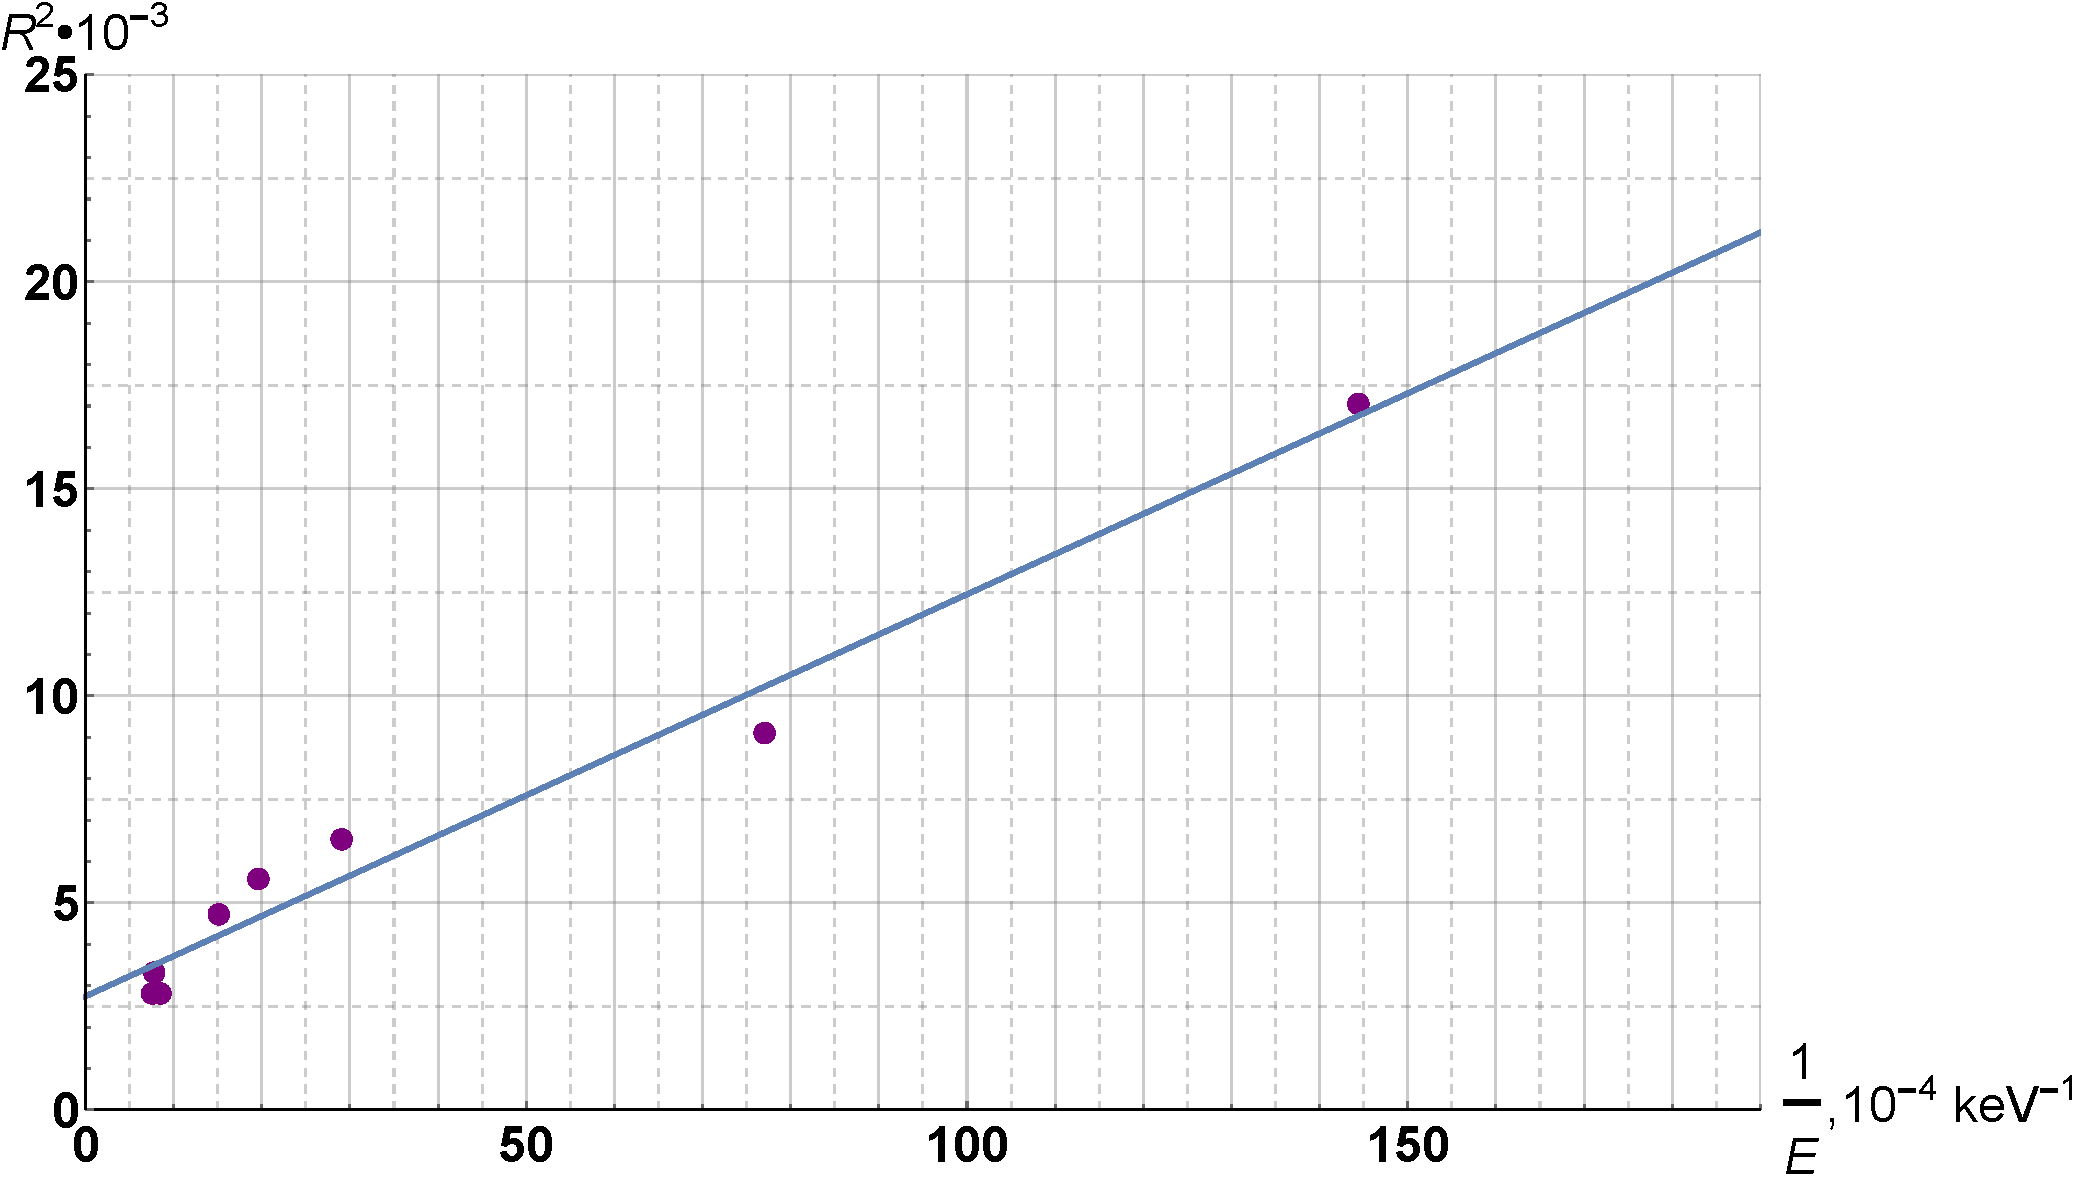
\includegraphics[scale=0.5]{r^2.pdf}
		\caption{Проверка формулы $ R = \dfrac{\mathrm{const}}{E} $}
	\end{figure} 

Результаты фита сведем в таблицу:

\begin{table}[H]
	\caption{Фит рис. 9 функцией $ y = ax + b $}
	\begin{center}
		\begin{tabular}{|c|c|c|}
			\hline
			& \text{Estimate} & \text{Standard Error} \\
			\hline
			b & 2.74367 & 0.40169 \\
			a & 0.097081 & 0.00673854 \\
			\hline 
		\end{tabular} 
	\end{center}
	\label{r2_fit}
\end{table}

Видно, что точки вполне хорошо описывают прямую.

Теперь найдем пики обратного рассеяния. 

\begin{table}[H]
	\caption{Комптновские спектры}
	\begin{center}
		\begin{tabular}{|c|c|c|}
			\hline 
			Образец & $ E_i, $ кэВ  & $ E_{обр}, $ кэВ  \\
			\hline 
			Натрий $ \mathrm{^{22}Na} $  & 511.4 & 190 \\
			Цезий $ \mathrm{^{137}Cs} $ & 661.5 & 205 \\
			Кобальт $ \mathrm{^{60}Co} $ & 1328.1 & 230 \\
			Европий	 $ \mathrm{^{152}Eu} $ & 129.973 & 95 \\
			Европий	 $ \mathrm{^{152}Eu} $& 343.172 & 170 \\
			\hline 
		\end{tabular} 
	\end{center}
	\label{obr}
\end{table}

Построим график зависимости $ E_{обр} = f(E) $ и профитируем его согласно \eqref{Eobr}:

	\begin{figure}[H]
	\label{graf_obr}
	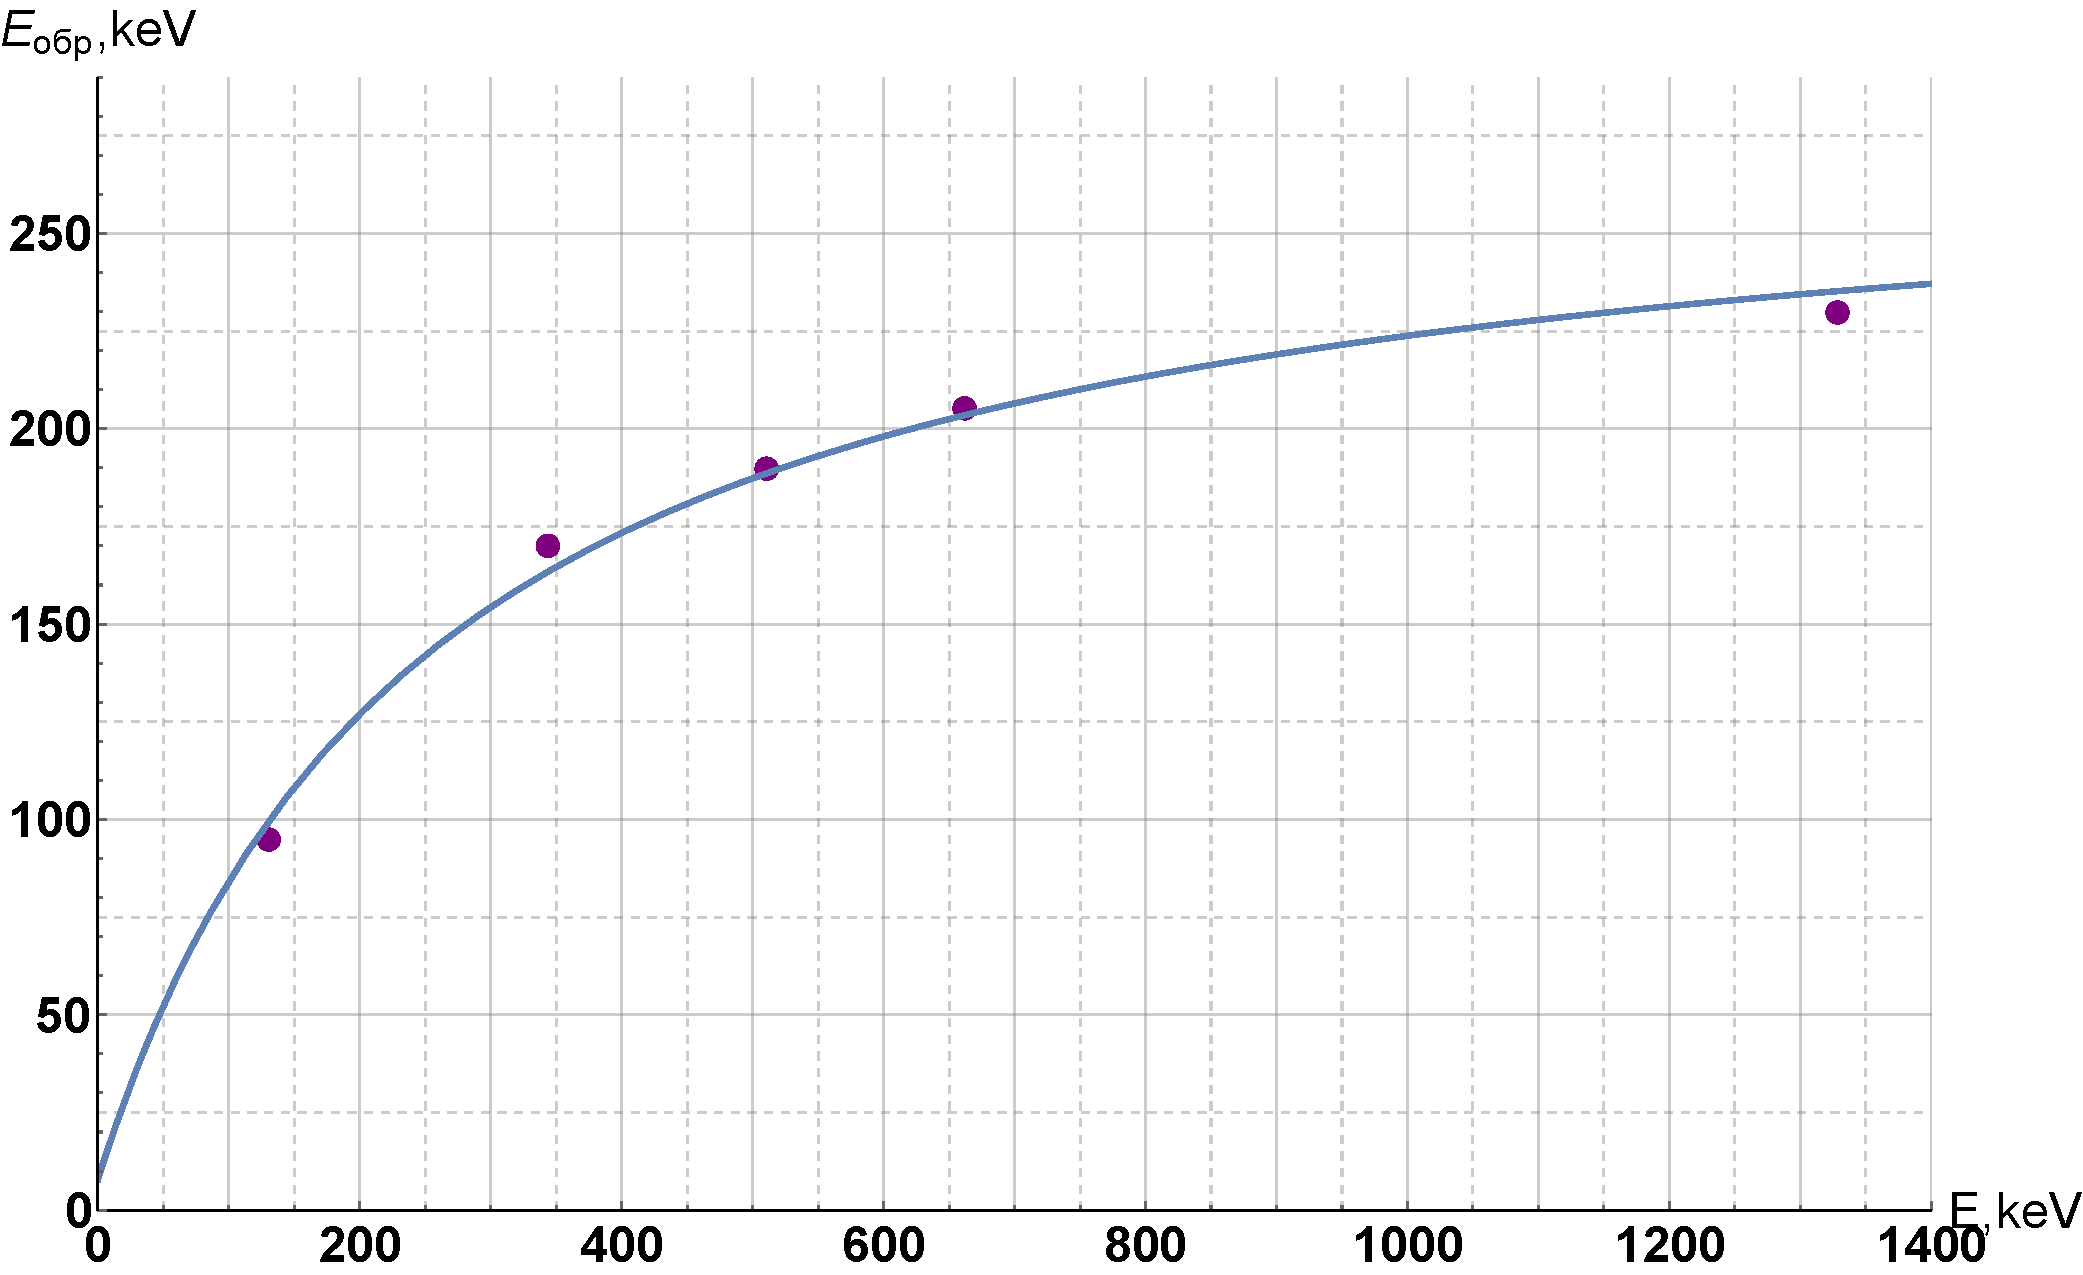
\includegraphics[scale=0.45]{ee.pdf}
	\caption{Проверка формулы $ R = \dfrac{\mathrm{const}}{E} $}
\end{figure} 

Результаты фита сведем в таблицу:

\begin{table}[H]
	\caption{Фит рис. 10 функцией $ y = a \dfrac{x}{1 + \dfrac{x}{255}} + с $}
	\begin{center}
		\begin{tabular}{|c|c|c|}
			\hline
			& \text{Estimate} & \text{Standard Error} \\
			\hline
			a & 1.06274 & 0.0584254 \\
			c & 7.85222 & 9.68542 \\
			\hline 
		\end{tabular} 
	\end{center}
	\label{obr_fit}
\end{table}

Заметим, что на наших графиках в левой части спектра присутствует узкий пик, соответствующий энергии порядка $ E_x \simeq 40 - 100 $ кэВ. Это соответствует характеристическому излучению из свинца, служащего защитой спектрометра от внешнего излучения. 

Пронаблюдав на осциллографе изображение импульсов с ФЭУ, оценим величины $ \tau_0 \simeq 0.4 $ мкс --- характерное время высвечивания для ФЭУ, и постоянную времени $ RC \simeq 3 $ мкс. Это было оценено по передним и задним фронтам импульсов соответственно. 
	
%	\section{Вывод }
	
\end{document}
